\chapter{Estado del arte}
\label{ch:chap02}

\section{Modelos de iluminación}
\label{sec:dibujado}

El proceso de dibujado de gráficos por computadora comprende la generación automática de imágenes a partir de tres parámetros principales,
un observador, superficies geométricas que representan objetos de la realidad y las propiedades físicas de los materiales que los componen.
Trivialmente, esto puede ser reducido al problema de cálculo del valor de intensidad lumínica observada en un punto $x$ y proveniente de
otro punto $x'$. Matemáticamente, este problema fue planteado por \citeauthor{Kajiya} en \citeyear{Kajiya}, comunmente nombrado
denominado <<la ecuación del rendering>>:

\begin{equation}
    I(x,x') = g(x,x') \bigg[\epsilon(x,x') + \int_{S} \rho(x,x',x'')I(x',x'') \delta x''\bigg] \label{eq:rendering}
\end{equation}
donde:
\begin{itemize}
    \item $I(x,x')$ describe energía de radiación lumínica obsrvada en el punto $x$ proveniente de $x''$
    \item $g(x,x')$ es un término geométrico, toma el valor de $0$ si existe oculsión entre $x'$ y $x$ en otro caso su valor es $\dfrac{1}{r^{2}}$ donde $r$ es la distancia entre $x'$ y $x$
    \item $\epsilon(x,x')$ mide la energía emitida por la superficie en el punto $x'$ a $x$
    \item $\int_{S} \rho(x,x',x'')I(x',x'') \delta x''$ está compuesta por dos términos:
        \begin{itemize}
            \item $\rho(x,x',x'')$ es el término de dispersión de la luz que llega desde $x''$ a $x$ desde el punto $x'$
            \item $I(x',x'')$ describe energía de radiación lumínica observada en el punto $x'$ proveniente de $x''$
        \end{itemize}
    por lo que este término refiere a la intensidad percibida desde $x$ considerando todos las reflexiones de
    luz posibles para el espacio $S$.
\end{itemize}

Existen distintos métodos de resolución de la ecuación del rendering, la mayoría implican aproximaciones dado el gran costo 
computacional requerido para calcular el valor exacto de $I(x,x')$. Estos métodos balancean el costo computacional de los algoritmos
utilizados y la fidelidad con el valor final de la función. Dependiendo de las decisiones y simplificaciones consideradas
existen dos clasificaciones posibles para el modelo: local y global \label{local-vs-global-img}.

\begin{minipage}[h]{0.8\linewidth}
    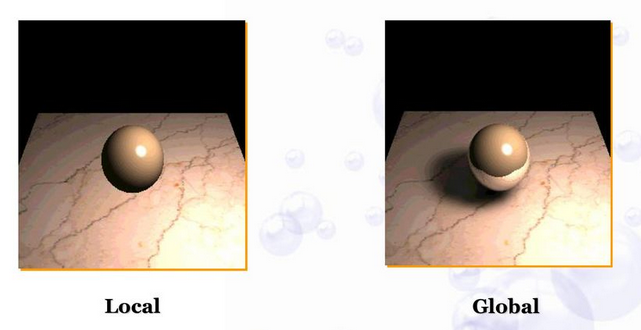
\includegraphics[width=\linewidth]{assets/local_vs_global}
    \captionof{figure}{Dibujado utilizando iluminación local y global}
    \label{local-vs-global-img}
\end{minipage}

\section{Iluminación local}
\label{sec:ilumlocal}
Los modelos de iluminación local como el propuesto por \citeauthor{Phong} en \citeyear{Phong} tienen en cuenta las propiedades físicas de los materiales
y las superficies de cada uno de los objetos de la escena de forma individual. Es decir, al dibujar uno de los
objetos no se toman en cuenta las posibles interacciones de los haces de luz con los objetos restantes.

En referencia a la ecuación del rendering, el término
geométrico nunca toma el valor 0 es decir, no se toma en cuenta las colisiones de los haces de luz con otros
objetos, $\epsilon(x,x')$ toma un valor constante (independiente de $x'$) y $\int_{S} \rho(x,x',x'')I(x',x'') \delta x''$ toma el valor constante $1$.

\section{Iluminación Global}
\label{sec:ilumglobal}

El término iluminación global refiere a una modelo de
computación gráfica que simula completamente las interacciones de la luz con todos los objetos que se encuentran 
en la escena. Es decir, en contraposición a la iluminación local, se consideran los fenómenos de
reflexión y refracción de la luz.

\section{Radiosidad}
\label{sec:radiosidad}

El transporte de la luz entre superficies puede ser modelado a través de la propiedad física conocida como
la radiosidad, definida como el flujo de energía irradiada por unidad de área. 

Oroginalmente, este modelo de iluminación global fue propuesto por \citeauthor{Goral} en \citeyear{Goral} se basa en modelos matemáticos
similares a los que resuelven el problema de la transferencia de calor en sistemas cerrados, conocidos como métodos de elementos finitos.

\subsection{Radiosidad en superficies lambertianas}

La solución propuesta por \citeauthor{Goral} implica que todas las superficies son idealmente lambertianas. Además considerara
que cada superficie irradia energía lumínica en todas direcciones en un diferencial de área $\delta_{A}$, para una dirección de vista $\omega$ puede ser definida como:

\begin{equation}
    i = \frac{\delta{P}}{\cos{\phi\delta\omega}} \label{eq:i}
\end{equation}
donde:
\begin{itemize}
    \item $i$ es la intensidad de la radiación para un punto de vista particular
    \item $\delta{P}$ es lae energía de la radiación que hemana la superficie en al dirección $\phi$ con ángulo sólido $\delta\omega$
\end{itemize}

En superficies perfectamente lambertianas, la energía reflejada puede ser expresada como: $\frac{\delta{P}}{\delta{\omega}} = k\cos{\phi}$. Donde $k$ es una constante.
Sustituyendo en \eqref{eq:i} se obtiene: $\frac{\delta{P}}{\delta{\omega}} = \frac{k\cos{\phi}}{\cos{\phi}} = k$, esto implica que la energía percibida de un punto $x$ 
es constante, independientemenete del punto de vista.

Es por esto que la energía total que deja una superficie ($P$) puede ser calculada integrando la energía que deja la superficie en cada dirección posible,
esto es, se integra la energía saliente en un hemiesfera centrada en el punto estudiado:

\begin{equation}
    P = \int_{2\pi} \delta{P} = \int_{2\pi} i\cos{\phi}\delta{\omega} = i \int_{2\pi} \cos{\phi}\delta{\omega} = i\pi \label{eq:P}
\end{equation}

Por tanto, dada una superficie $S_{i}$, es posible calcular la energía lumínica que deja la superficie utilizando \eqref{eq:P}.
Resta definir la \textit{cerradura} de una superficie, definiremos la cerradura de una superficie como los límites que definien
los puntos internos y externos de esta. Esto hace que el problema sea resoluble utilizando métodos de elementos finitos, con esta reformulación 
del problema, es fácilmente trasladable a la ecuación \eqref{eq:rendering}.

\begin{equation}
    B_{j} = E_{j} + \rho_{j} \sum_{i=1}{N} B_{i} F_{ij} \label{eq:radiosity}
\end{equation}
donde:
\begin{itemize}
    \item $B_{j}$ es la intensidad lumínica (radiosidad) que deja la superficie $j$.
    \item $E_{j}$ es la intensidad lumínica directamente emitida por $j$.
    \item $\rho_{j}$ es la reflectividad del material para la superficie $j$.
    \item $F_{ij}$ se denomina \textit{factor de forma}, un término que representa la fracción de energía lumínica
    que deja la superficie $i$ y llega a $j$. 
\end{itemize}

Cabe destacar que la naturaleza recursiva de la ecuación anterior, implica que se toman en cuenta todas las reflexiones 
difusas que existan en la escena. Como puede observarse, resolver el sistema de $N$ ecuaciones lineales 
bastaría para conocer la energía emitida por cada superficie cerrada. 

$\mathbf{E}$, $\mathbf{\rho}$ dependen de los materiales que compongan la escena, son parámetros dados. Sin embargo, 
resta computar la matriz de factores de forma $\textbf{F}$ para finalmente obtener el vector de radiosidades $\textbf{B}$. 
Para determinar una entrada de la matriz $F_{ij}$ involucrando a las superficies $i$ y $j$ de área $A(i)$, $A(j)$,
considerando los diferenciales infinitesimales de área $\delta{A_{i}}$, $\delta{A_{j}}$ el ángulo sólido visto por
$\delta{A_{i}}$ es $\delta{\omega} = \frac{\cos{\phi_{j}\delta{A_{j}}}}{r^{2}}$. Susituyendo en \eqref{eq:P} se obtiene:

\begin{equation}
    \delta{P}_{i}\delta{A_{i}} = i_{i} \cos{\phi_{i}}\delta{\omega}\delta{A_{i}} = \frac{P_{i}\cos{\phi_{i}}\cos{\phi_{j}}\delta{A_{i}}\delta{A_{j}}}{\pi r^{2}}
\end{equation}

Considerando que ${P}_{i}{A_{i}}$ es la energía que deja $i$, y que el factor de forma $F_{ij}$ representa el porcentaje
de dicha energía que llega a $j$ podemos observar que:

\begin{equation}
    F_{\delta{A_{i}}-\delta{A_{j}} = \frac{\frac{P_{i}\cos{\phi_{i}}\cos{\phi_{j}}\delta{A_{i}}\delta{A_{j}}}{\pi r^{2}}}{P_{i}\delta{A_{i}}} = \frac{\cos{\phi_{i}}\cos{\phi_{j}}\delta{A_{i}}}{\pi{r^{2}}}
\end{equation}

Integrando, para obtener el factor de forma para el área total:

\begin{equation}
    F_{ij} = \frac{1}{A_{i}} \int_{A_{i}}\int_{A_{j}}\frac{\cos{\phi_{i}}\cos{\phi_{j}}\delta{A_{i}}\delta{A_{j}}}{\pi{r^{2}}} \label{eq:ff}    
\end{equation}

De \eqref{eq:ff} se obtienen las siguientes propiedades:
\begin{enumerate}
    \item $A_{i}F_{ij} = A_{j}F{ji}$
    \item $\sum_{j=1}^{N} F_{ij} = 1$
    \item $F_{ii} = 0$
\end{enumerate}

\section{Rasterización}
\label{sec:rasterizacion}

\subsection{OpenGL}
\label{sec:opengl}

\section{Raytracing}
\label{sec:raytracing}

\subsection{Embree}
\label{sec:embree}
